\clearpage

\section{Das Zufallsexperiment}

Das Zufallsexperiment, dass wir betrachten, ist das Auftreffen von Photonen auf Strahlteiler verschiedener Anzahl mit verschiedenen Durchlasswahrscheinlichkeiten. Hierbei nehmen wir an das immer acht Photonen ausgelöst werden und in unser Experiment gelangen. Nun lassen wir die Photonen hintereinander auf die Strahlteiler treffen und untersuchen wie viele Photonen durch alle Strahlteiler gelangt sind. Hierbei ist die Durchlasswahrscheinlichkeit für ein Photon bei allen Strahlteilern gleich. Diesen Versuch führen wir nun für einen, drei und fünf Strahlteiler durch mit Durchlasswahrscheinlichkeiten von ein Viertel, ein Halb und Dreiviertel und das jeweils 500.000.000 Mal und untersuchen dabei die Verteilung der am Ende von allen Strahlteilern durchgelassenen Photonen.

\subsection{Methode der Durchführung}

Wir haben diesen Versuch mithilfe von Java simuliert. Im Anhang ist der Java-Code vorzufinden den wir zur Simulation benutzt haben.\\
Unserer Programm zur Simulation des Zufallsexperimentes benötigt als Argumente als erstes die Anzahl der Photonen, in unserem Fall acht, dann die Anzahl der Strahlteiler, die Durchlasswahrscheinlichkeit und die Anzahl der Durchführungen des Experimentes, sowie wahlweise den Dateinamen mit Dokumententyp unter dem die Daten abgespeichert werden soll. In diesem Fall werden die Daten nicht ausgegeben, sondern nur als Dokument gespeichert.\\
Hierbei lassen wir das Programm als erstes testen ob genug Argumente vorhanden sind, sonst gibt es eine Fehlermeldung aus. Als nächstes initialisieren wir die Variablen unseres Programmes als ganze Zahlen beziehungsweise die Wahrscheinlichkeit als Kommazahl. Zusätzlich definieren wir uns die Liste absHaeufigkeit die um eins länger ist als wir Photonen in unser Experiment schicken und die wir benutzen um unsere absoluten Häufigkeiten zu erhalten.\\
Dann verwenden wir eine For-Schleife die von Null bis zur Anzahl der Durchführungen läuft und nPhotonen gleich unserer Startphotonenzahl setzt. Nun wenden wir in einer inneren For-Schleife, die die Anzahl der Strahlteiler durchläuft, eine Funktion Strahlenteiler auf nPhotonen an und erhalten als Output dieser For-Schleife die Anzahl der durchgelassenen Photonen von dieser Durchführung des Zufallsexperiments. Zum Abschluss erhöhen wir nun in der äußeren For-Schleife an der Stelle unserer Liste absHaeufigkeit, die gleich unserem nach der Durchführung der inneren For-Schleife erhaltenen nPhotonen ist, den Wert um Eins. Hierbei ist es hilfreich, dass Listen in Java mit dem nullten Element beginnen, wodurch wir als das nullte Listenelement das absolute Häufigkeit von Null durchgelassenen Photonen haben können etc. Dies führen wir nun so oft durch wie wir angegeben haben und erhalten so eine Liste mit unseren absoluten Häufigkeiten für unserer Zufallsexperiment.\\
Als nächstes testen wir mit einem If-Befehl, ob wir das Ergebnis als Dokument speichern sollen oder einfach ausgeben sollen, indem wir die Anzahl unserer Argumente untersuchen.\\
Als vorletztes definieren wir noch unsere bereits verwendete Funktion Strahlenteiler, wobei wir als erstes unseren Output sout Null setzen, dann durchlaufen wir mit einer For-Schleife alle Photonen die wir in den Strahlteiler schicken und generieren für jedes eine Zufallszahl zwischen Null und Eins und testen ob diese kleiner oder gleich unserer festgelegten Wahrscheinlichkeit ist. Wenn dem so ist erhöhen wir sout um Eins, sonst nicht. Zum Schluss definieren wir noch die Funktion, die unsere Output-Datei generiert. Hierbei durchlaufen wir mit einer For-Schleife unsere Liste absHaufigkeit und schreiben diese in die entsprechende Zeile des Dokuments in der Form „durchgekommene Photonen“; “absolute Häufigkeit“.


\section{Auswertungen}

\subsection{Diagramme}
\subsubsection{Ein Strahlteiler}


\begin{center}
	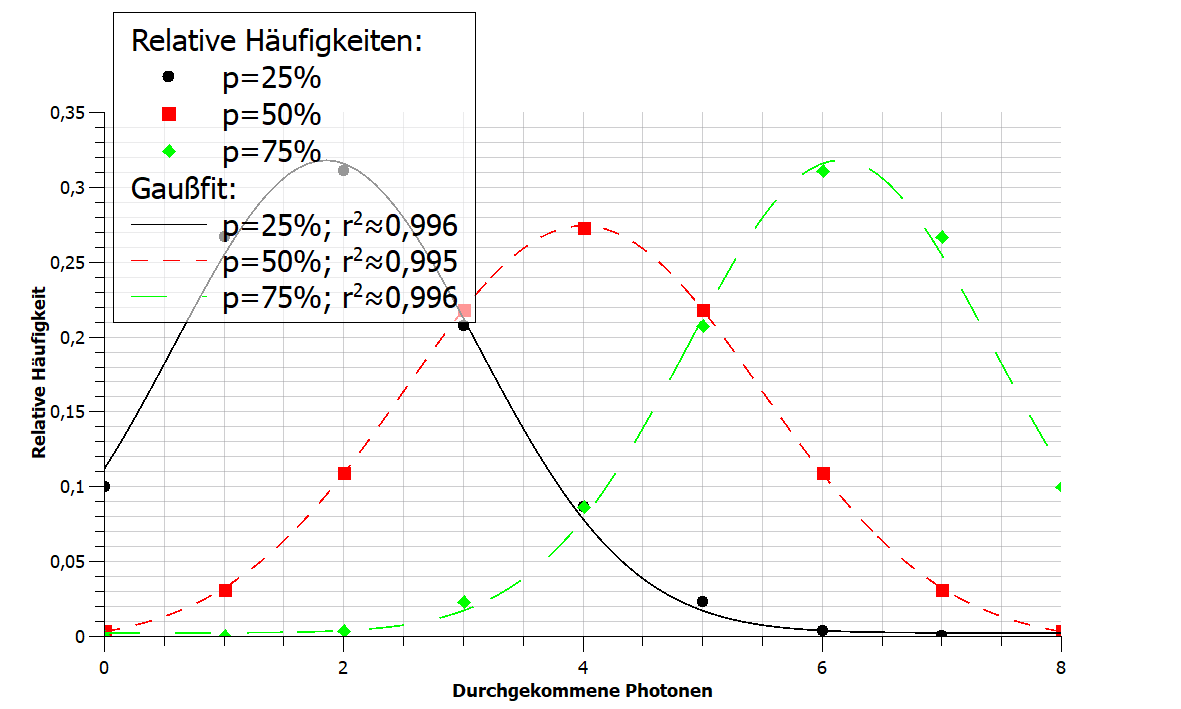
\includegraphics{IMAGE/1ST}
	\captionof{figure}{Dargestellt sind die relativen Häufigkeiten aufgetragen gegen die  durchgekommenen Photonen, bei einem Strahlteiler. Es wurden 500 Millionen Versuche durchgeführt.}
\end{center}
\vspace{-1cm}
\subsubsection{Drei Strahlteiler}

\begin{center}
	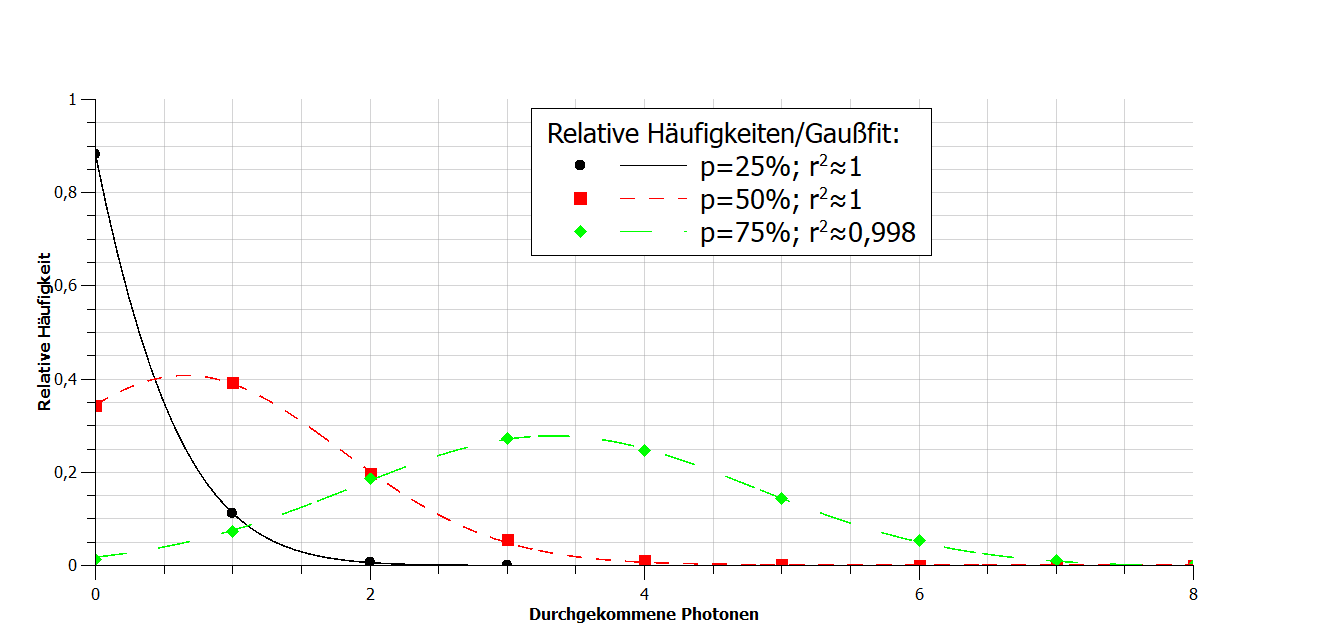
\includegraphics{IMAGE/3ST}
	\captionof{figure}{Dargestellt sind die relativen Häufigkeiten aufgetragen gegen die  durchgekommenen Photonen, bei drei Strahlteilern. Es wurden 500 Millionen Versuche durchgeführt.}
\end{center}

\subsubsection{Fünf Strahlteiler}

\begin{center}
	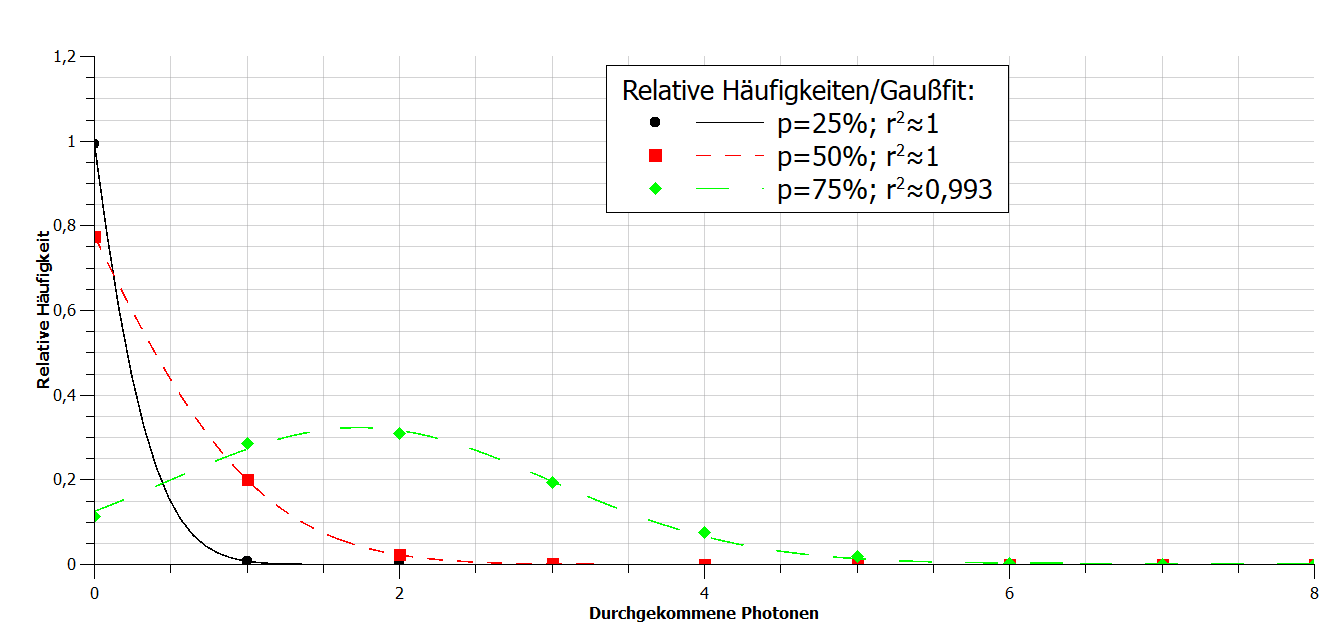
\includegraphics{IMAGE/5ST}
	\captionof{figure}{Dargestellt sind die relativen Häufigkeiten aufgetragen gegen die  durchgekommenen Photonen, bei fünf Strahlteilern. Es wurden 500 Millionen Versuche durchgeführt.}
\end{center}
\clearpage
\subsection{Analyse}
 
 Dies sind die verwendeten Formel:\\
 
 Binomialvereilung(n: Anzahl Versuche, P: Wahrscheinlichkeit Erfolg, k: Untersuchter Wert):\\
\begin{equation*}
 	P(X= k) = \binom{n}{k}p^k(1-p)^{n-k}
\end{equation*}

Normalverteilung($\sigma^2$:Varianz, $\mu$: Erwartungswert, x: Untersuchter Wert):\\
\begin{equation*}
	P(X= x) = \frac{1}{\sqrt{2\pi\sigma^2}}e^{-\frac{(x-\mu)^2}{2\sigma^2}},\qquad \mu = \sum_{i=1}^k x_i\cdot p_i, \qquad \sigma^2 = n\cdot p \cdot(1-p)
\end{equation*}

Poissonverteilung($\lambda$):\\
\begin{equation*}
	P(X=k)= \frac{\lambda^k}{k!}e^{-\lambda}
\end{equation*}

Da im folgendem nicht gefittet wurde, muss der $r^2$-Wert manuel ausgerechnet werden::\\
\begin{equation*}
	r^2 = 1- \frac{\sum_{i=1}^n(x_i-P(X=x))^2}{\sum_{i=1}^n(x_i-\overline{x})^2}, \qquad \overline{x}=\tfrac{1}{n}\sum_{i=1}^n x_i
\end{equation*}

\begin{center}
	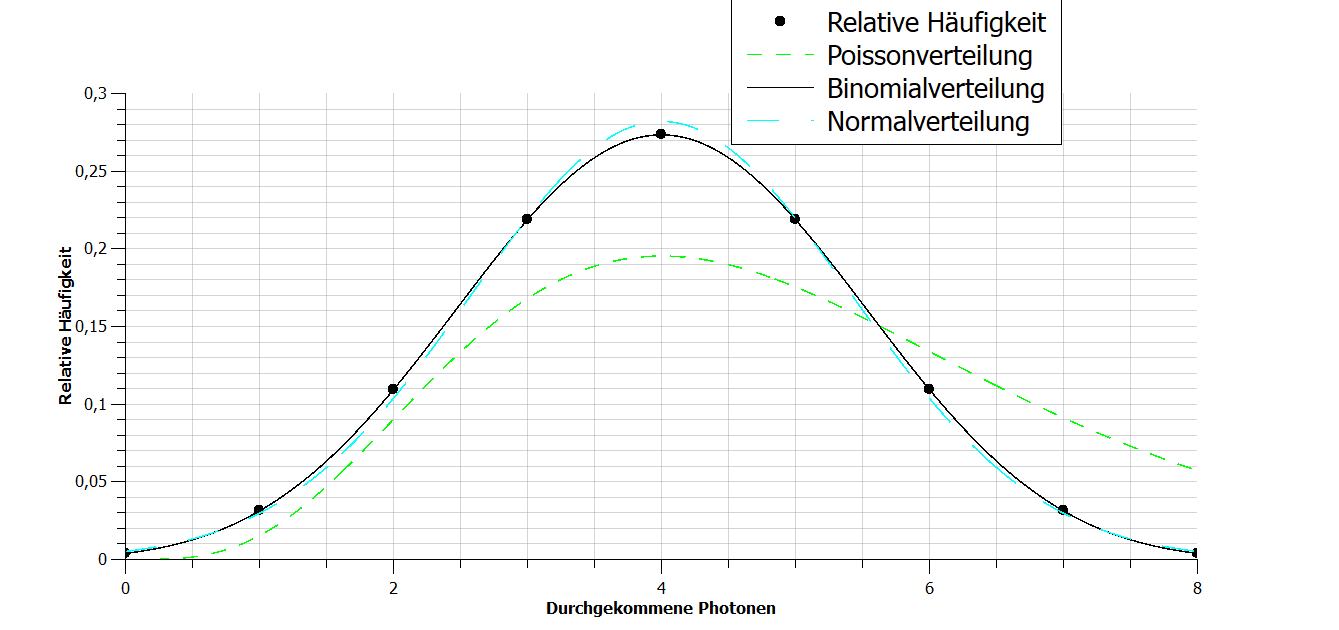
\includegraphics{IMAGE/1ST-P50}
	\captionof{figure}{Relative Häufigkeit aufgetragen auf durchgekommene Photonen, angenähert durch Poisson-, Binomial- und Normalverteilung Es wurde 1 Strahlteiler mit einer Durchlasswarscheinlichkeit von 50\% simuliert und 500 Millionen Versuche durchgeführt.\\ $r^2$: Poisson $\approx$ 0,79; Normal $\approx$ 0,998; Binom $\approx$ 1}
\end{center}
\clearpage
In diesem Diagramm ist deutlich zu erkennen, dass unser Zufallsexperiment keiner Poissonverteilung folgt. Des Weiteren ist zu erkennen, dass eine Normalverteilung durchaus als gute Näherung betrachtet werden kann. Es ist aber auch sichtbar das bei diesen Versuchsparametern eine Binomialverteilung die höchste Übereinstimmung vorzuweisen hat. Dies legt die Vermutung nahe das unser Zufallsexperiment auch ein Bernoulli-Versuch ist.

\begin{center}
	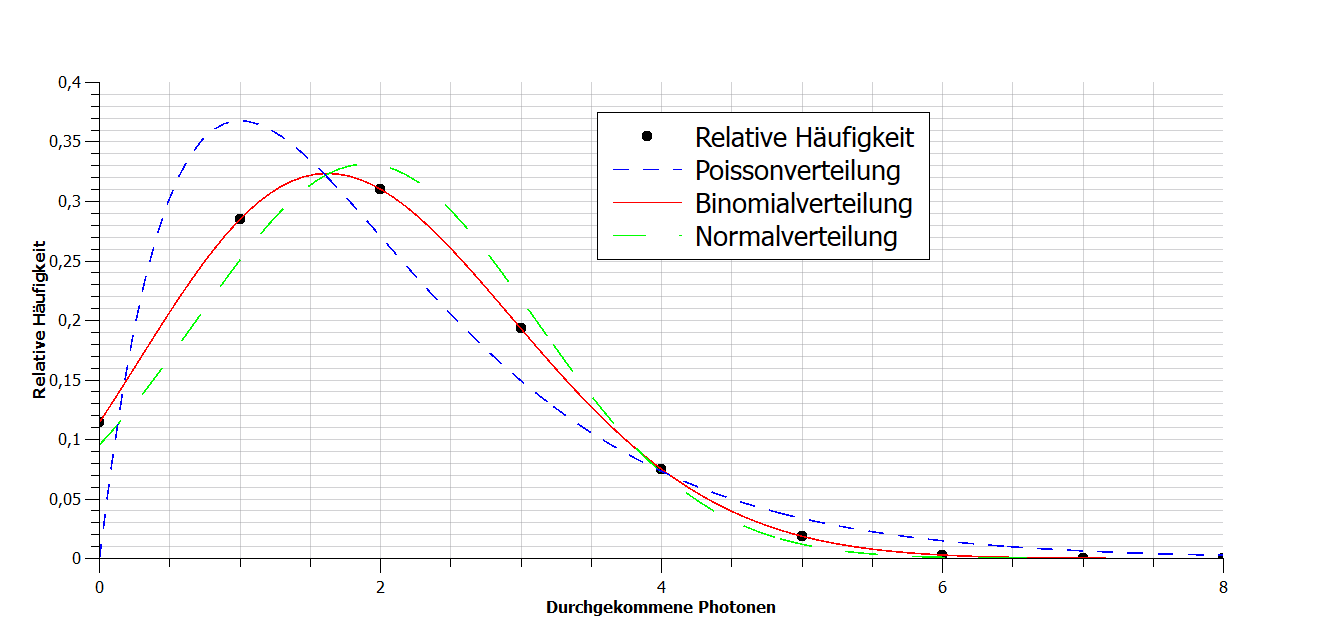
\includegraphics{IMAGE/5ST-P75}
	\captionof{figure}{Relative Häufigkeit aufgetragen auf durchgekommene Photonen, angenähert durch Poisson-, Binomial- und Normalverteilung Es wurden 5 Strahlteiler mit einer Durchlasswarscheinlichkeit von 75\% simuliert und 500 Millionen Versuche durchgeführt.\\ $r^2$: Poisson $\approx$ 0,8; Normal $\approx$ 0,98; Binom $\approx$ 1}
\end{center}

Es ist zu erkennen dass auch bei diesen Versuchsparametern dieselbe Beobachtung getätigt werden kann wie bei Diagramm 4, nämlich dass eine Binomialverteilung eines Bernoulli-Versuchs der Kettenlänge acht vorliegt.
Damit haben wir eine Übereinstimmung zwischen Theorie und Experiment, da man aus unserem Versuchsaufbau auf eine Binomialverteilung schließen kann. Da man bei einem Bernoulli-Versuch nur zwei Auskomm-Möglichkeiten hat, bei uns durchkommen oder nicht, und dann die Anzahl der Treffer, bei uns die Anzahl der durchgekommenen Photonen, untersucht, ist unser Zufallsexperiment in der Theorie ein Bernoulli-Versuch und dies wurde durch die Ausführung des Zufallsexperiments bestätigt.



\subsection{Zusammenfassung}
Zusammenfassend lässt sich über dieses Experiment sagen, dass es in diesem Fall eine hohe Übereinstimmung des theoretischen und des experimentellen Ergebnisses gibt. Abschließend  sei nur noch gesagt, dass es sicherlich für die Größe der Übereinstimmung, die wir erreicht haben, ein Vorteil war, dass wir zu jeder Konfiguration unserer Versuchsparameter 500 Millionen Durchführungen durchgeführt haben, da sich so Abweichungen besser wieder rausmitteln konnten.

\clearpage
\section{Anhang}

\subsection{Code}

\lstinputlisting{CONTENT/PhotonSim.java}

\subsection{Werte}

\begin{tabular}{|l|l|l|l|l|l|l|}
	\hline
	\multicolumn{7}{|c|}{1 Strahlteiler} \\\hline
	&\multicolumn{2}{|c|}{25\% Durchlass}&\multicolumn{2}{c|}{50\% Durchlass}&\multicolumn{2}{c|}{75\% Durchlass}\\\hline
	\#DP & ABS & REL  & ABS & REL & ABS & REL \\\hline
	0&50.060.590&0,10012118&1.952.901&0,003905802&7.793&1,5586e-05\\
	1&133.481.859&0,266963718&15.621.636&0,031243272&183.433&0,000366866\\
	2&155.705.375&0,31141075&54.684.469&0,109368938&1.922.575&0,00384515\\
	3&103.843.189&0,207686378&109.374.310&0,21874862&11.533.646&0,023067292\\
	4&43.260.603&0,086521206&136.733.468&0,273466936&43.254.905&0,08650981\\
	5&11.535.075&0,02307015&109.362.826&0,218725652&103.817.466&0,207634932\\
	6&1.922.542&0,003845084&54.692.025&0,10938405&155.734.561&0,311469122\\
	7&183.095&0,00036619&15.626.048&0,031252096&133.482.836&0,266965672\\
	8&7.672&1,5344e-05&1.952.317&0,003904634&50.062.785&0,10012557\\
	\hline
\end{tabular}

\begin{tabular}{|l|l|l|l|l|l|l|}
	\hline
	\multicolumn{7}{|c|}{3 Strahlteiler} \\\hline
	&\multicolumn{2}{|c|}{25\% Durchlass}&\multicolumn{2}{c|}{50\% Durchlass}&\multicolumn{2}{c|}{75\% Durchlass}\\\hline
	\#DP & ABS & REL  & ABS & REL & ABS & REL \\\hline
	0&440.816.470&0,88163294&171.803.814&0,343607628&6.238.437&0,012476874\\
	1&55.973.348&0,111946696&196.339.304&0,392678608&36.428.388&0,072856776\\
	2&3.109.143&0,006218286&98.188.913&0,196377826&93.022.782&0,186045564\\
	3&99.084&0,000198168&28.042.870&0,05608574&135.767.124&0,271534248\\
	4&1.930&3,86e-06&5.010.695&0,01002139&123.848.086&0,247696172\\
	5&25&5e-08&571.731&0,001143462&72.299.885&0,14459977\\
	6&0&0&41.039&8,2078e-05&26.389.380&0,05277876\\
	7&0&0&1.607&3,214e-06&5.504.504&0,011009008\\
	8&0&0&27&5,4e-08&501.414&0,001002828\\
	\hline
\end{tabular}

\begin{tabular}{|l|l|l|l|l|l|l|}
	\hline
	\multicolumn{7}{|c|}{5 Strahlteiler} \\\hline
	&\multicolumn{2}{|c|}{25\% Durchlass}&\multicolumn{2}{c|}{50\% Durchlass}&\multicolumn{2}{c|}{75\% Durchlass}\\\hline
	\#DP & ABS & REL  & ABS & REL & ABS & REL \\\hline
	0&496.109.350&0,9922187&387.855.414&0,775710828&57.255.964&0,114511928\\
	1&3.877.288&0,007754576&100.085.542&0,200171084&142.504.954&0,285009908\\
	2&13.333&2,6666e-05&11.300.032&0,022600064&155.176.959&0,310353918\\
	3&29&5,8e-08&728.933&0,001457866&96.568.486&0,193136972\\
	4&0&0&29.295&5,859e-05&37.552.673&0,075105346\\
	5&0&0&776&1,552e-06&9.350.079&0,018700158\\
	6&0&0&8&1,6e-08&1.456.188&0,002912376\\
	7&0&0&0&0&129.671&0,000259342\\
	8&0&0&0&0&5.026&1,0052e-05\\
	\hline
\end{tabular}
